\documentclass[a4paper, 12pt]{article}

\usepackage[top= 0.5in]{geometry}
\usepackage[utf8]{inputenc}
\usepackage[portuguese]{babel}
\usepackage{indentfirst}
\usepackage{graphicx}

\usepackage{biblatex}
\addbibresource{referencias.bib}

\title{IF668 - Introdução à Computação}
\author{Samuel Alves Marsaro}
\date{Dezembro, 2021}

\begin{document}

\maketitle


\section{Introdução}
\par
Primeiramente, pode-se afirmar que a cadeira de Introdução à Computação é basicamente aquela que dará ao aluno a base de tudo aquilo que envolve a computação no geral, introduzindo-o a conceitos não muito comuns na sociedade, como Engenharia de Software, Inteligência artificial e Teoria da computação.\cite{sitecinIC}
\par
\begin{figure}[h]
    \centering
    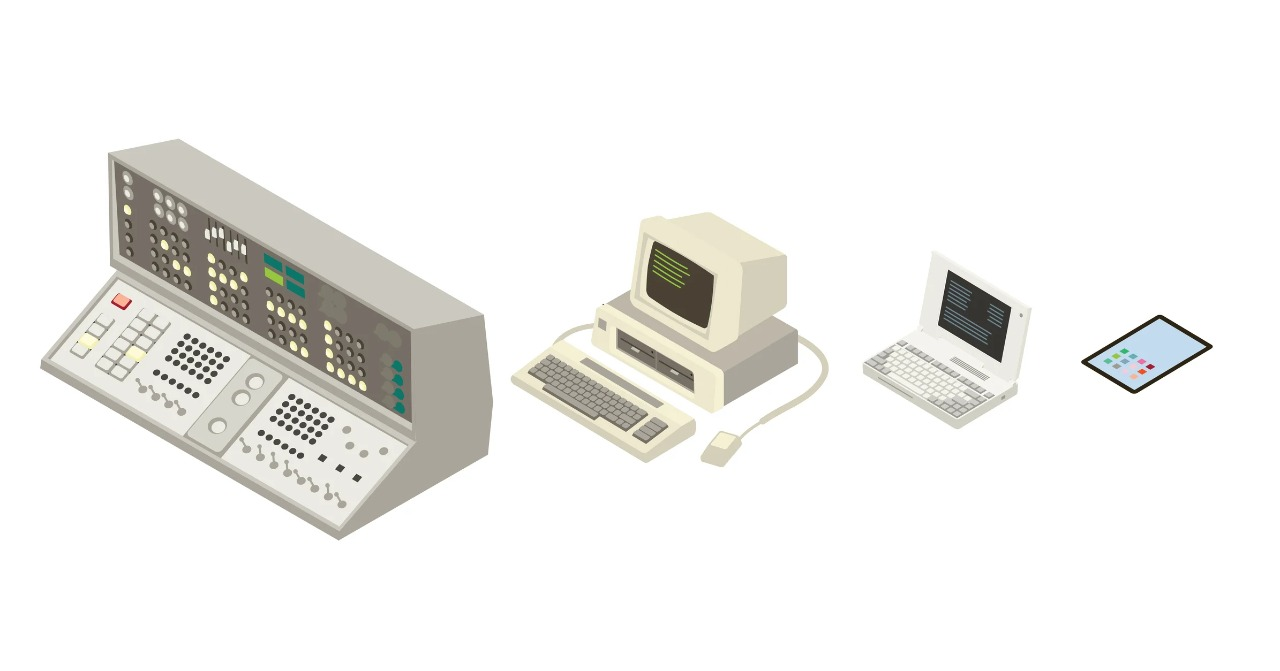
\includegraphics[width=1\textwidth]{Imagens/computadores.jpeg}
    \caption{Computadores ao longo da história\cite{artigo_computadores}}
    \label{fig:computadores}
\end{figure}
    
    
\section{Relevância}
    \par
A importância de tal disciplina se dá pelo fato da área da computação ser extremamente vasta e um tanto quanto subjetiva. Tal cadeira busca racionalizar e explicar essa subjetividade de tal maneira que seja possível que o universitário venha a escolher futuras cadeiras baseadas no que será melhor para ele, tendo uma base bem fomentada em tudo. Além disso, é perceptível o quanto é importante que se tenha uma introdução boa do conceito da evolução dos computadores para cadeiras como Historia e Futuro da Computação.


\section{Relação com outras disciplinas}
    \par
    \begin{itemize}
        \item IF690- HISTORIA E FUTURO DA COMPUTACAO
            \par 
            Além de pré-requisito, é fundamental que se tenha tido uma base muito boa na cadeira de Introdução à Computação, a fim de facilitar o processo de adesão e andamento das aulas de história, já que nessa cadeira se estudam alguns eventos que impulsionaram a história da tecnologia.\cite{sitecinHFC}
        \item IF669- INTRODUCAO A PROGRAMACAO
            \par
            Como essa disciplina também é de conceito introdutório, ela é co-requisito da cadeira de Introdução à Computação, sendo muito importante a união das duas para o andamento fluido do período.\cite{sitecinIP}
    \end{itemize}

\printbibliography

\end{document}
